%----------------------------------------------------------------------------------------
%	PACKAGES AND THEMES
%----------------------------------------------------------------------------------------
\documentclass[aspectratio=169,xcolor=dvipsnames]{beamer}
\usetheme{Warsaw}

\usepackage{hyperref}
\usepackage{graphicx} % Allows including images
\usepackage{booktabs} % Allows the use of \toprule, \midrule and \bottomrule in tables
\graphicspath{ {./Images/} }
%----------------------------------------------------------------------------------------
%	TITLE PAGE
%----------------------------------------------------------------------------------------

% The title
\title[Introducing]
\subtitle{}

\author[Kasra M] {Kasra M}

\date{\today} % Date, can be changed to a custom date


%----------------------------------------------------------------------------------------
%	PRESENTATION SLIDES
%----------------------------------------------------------------------------------------

\begin{document}

\begin{frame}
    % Print the title page as the first slide
    \titlepage
\end{frame}
\begin{frame}{Inspiration?}
\begin{center}
    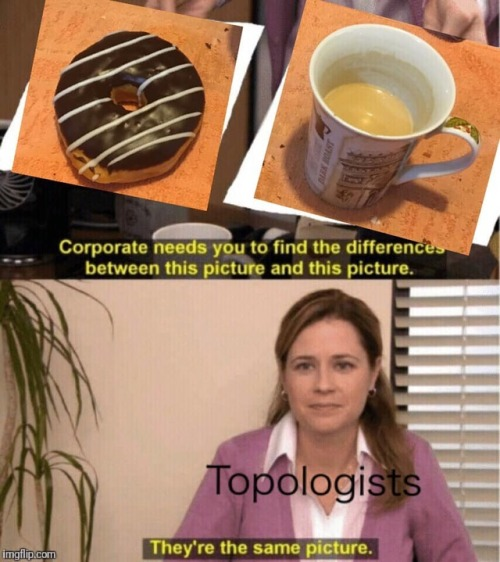
\includegraphics[scale = 0.25]{topology}
\end{center}
\end{frame}
\begin{frame}{Overview}
    % Throughout your presentation, if you choose to use \section{} and \subsection{} commands, these will automatically be printed on this slide as an overview of your presentation
    \tableofcontents
\end{frame}

%------------------------------------------------
\section{Introducing Continuity}
%------------------------------------------------

\begin{frame}{Continuity}
    The idea of continuity isn't well defined before analysis, and the definition changes. For example many people are told that a function is continuous if it can be graphed without picking up your pen. Topology offers us a much clearer definition of continuity: \newline
    \begin{block}{Definition}
        A function f from a topological space X to Y is continuous if for every $ V \subseteq Y$, $f^{-1}(V)$ is open in X
    \end{block}
\end{frame}
\section{Donut = Cup?}
\begin{frame}{Why Donut = Cup?}
    The infamous meme that claims topologist think that a donut is the same as a mug or cup. Well, the reality is that that is true, except possibly not in the way you would expect. The topological properties of the cup/mug and a torus(donut) are the same, so we introduce a concept called a homeomorphism.
\end{frame}
\begin{frame}{Homeomorphisms}
    A homeomorphism is very similar to a isomorphism from algebra, but where instead of preserving algebraic properties, the homeomorphism preserves topological properties like genus and compactness.\newline
    \begin{block}{Definition}
        A homeomorphism is a function $f:X \mapsto Y$, where X and Y are topological spaces, such that:
        \begin{enumerate}
            \item f is bijective 
            \item f is continuous
            \item $f^{-1}$ is continuous
        \end{enumerate}
    \end{block}
\end{frame}
\section{Defining a donut}
\begin{frame}{Introduction}
    In this next section, I will introduce the quotient topology, so that we can create the donut(torus), and examine some of its topological properties(and maybe even analyze what we can tell about a mug or cup from it).\newline
    The idea of an equivalence class(and relation) will be an important part in understanding the quotient topology: \newline
   \begin{block}{Definition}
          A binary relation, $\sim$, on a set X is said to be an equivalence relation if it satisfies certain conditions(for all $x,y,z \in X$):
          \begin{enumerate}
              \item $x \sim x$
              \item $x \sim y$ iff $y \sim x$
              \item if $x\sim y$ and $y\sim z$, $x\sim z$
          \end{enumerate}
   \end{block}
    
\end{frame}
\begin{frame}{Equivalence Class}
    \begin{block}{Definition}
           For some $x \in X$, an equivalence class is said to be the subset of X given by \newline
           [x] := $\{y \in X \mid x \sim y\}$ We can also define the set of all equivalence classes on X as:
           \newline $(X/ \sim) = \{[x] \mid x\in X\}$
    \end{block}
    Now, we can define the open set in ($X/\sim$) :
    \begin{block}{Definition}
           For some $U \subseteq (X/\sim)$, where X is a topological space and $\sim$ is an equivalence relation on it, U is open iff: \newline
           $\bigcup_{[x] \subseteq U} [x] \subseteq X$ is open in X
    \end{block}
    Here, we have created the quotient topology! We can confirm that this is indeed a topology
\end{frame}
\begin{frame}{Creating a Torus}
    To create a torus, we use the equivalence relation $(x,y)\sim (x+1,y) \sim (x, y+1)$ in the Cartesian plane. This is wonderful, but now we can analyze some of the topological properties of a torus.
    \begin{block}{Example Property}
           A torus is topologically compact, and therefore so is a mug. A compact space is one where any covering of the space has a finite subcover. 
    \end{block}
    
\end{frame}
\begin{frame}{End Notes}
We can use the idea of a quotient map to also build a quotient topology, but for the purpose of creating a torus, I used the method using equivalence classes:
\begin{block}{Definition}
       A surjective map $p:X \mapsto Y$, where X and Y are topological spaces, is said to be a quotient map if for $V \subseteq$ Y, V is open in Y iff $f^{-1}(V)$ is open in X
    \end{block} 
    using this idea, we can show that given a set A and a space X, there exists only one topology on A, relative to p that is, and this topology is called the topology induced by p
\end{frame}
\section{References}
\begin{frame}{References}
    Topology Second Edition. Munkres, James. Pearson Publishing
    \newline
    \newline
    Quotient Topology Supplement, http://www.math.ucsd.edu/$\sim$bprhoades/190w16/quotient.pdf
\end{frame}

\end{document}